\chapter{The View Panel}\label{lab:view}

The view panel allows the user to review recordings and adjust/create annotations to describe observed user behaviour.

\section{Overview}\label{lab:view_stimuli}

\begin{figure}[h]
\begin{center}
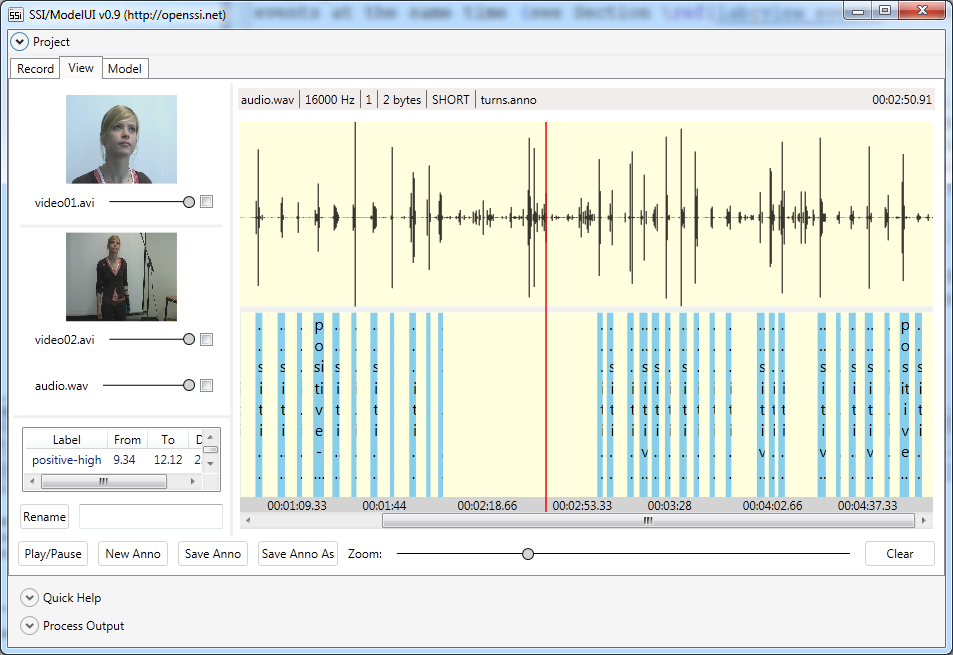
\includegraphics[scale=0.5]{pics/view_gui.png}
\end{center}
\vspace{-0.5cm}
\caption{The view panel.}
\label{fig:view_gui}
\end{figure}

The view panel has a time line for navigation through the recording (see Section \ref{lab:view_navigate}). To load the signals and annotations of a recording session double click the according recording. Videos are displayed on the left side together with a volume slider for each media. Events of the currently selected annotation track (yellow background) are listed in a table below the videos. It can be used to quickly jump to a certain event or change the label of several events at the same time (see Section \ref{lab:view_events}). The \texttt{Clear} button removes all signals and annotations from the panel.

\section{Navigation}\label{lab:view_navigate}

The current position in the time line is marked by a red cursor. Clicking on a track moves the cursor to that position. If at least one media (audio or video) has been loaded, playback is possible by pressing the \texttt{space bar}. Usually, the recording is played until the end of the timeline unless an event has been selected. In this case the recording is looped within the borders of the events. An event is selected by clicking on it. As long as replay is active the user cannot change the position of the cursor. Pressing the \texttt{ space bar} again stops replay. The slider on the navigation bar can be used to adjust the zoom level.

\section{Annotations}\label{lab:view_events}

Annotation files contain detected events. An event has a start and a stop time, as well as, a label string, which can be empty. An annotation file aggregates a set of events and is stored as a plain text file ending on \texttt{*.anno}, e.g.:

\begin{verbatim}
 8.9 13.5 labelA
16.0 19.6 labelB
21.6 24.8
27.2 30.7 labelA
\end{verbatim}

 Events of an annotation file are displayed as segment blocks on an annotation track. The label of an event is shown inside the box. new annotations can be created (\texttt{New}) and saved (\texttt{Save}, \texttt{Save As}). Right click on an annotation track adds a new event. By default the label is empty. Hitting the \texttt{enter key} allows the user to apply a string. Pressing the \texttt{del key} removes a selected event from the current annotation track. When the mouse is moved to the center of an event the cursor shape changes to a cross cursor. By holding the left mouse button pressed the event can now be moved along the track. Moving the mouse to the left or right border of an event allows the user to adjust its borders.
